\glsresetall
\chapter{Literature Review}
This chapter will aim to provide a critical evaluation of the current relevant research that was investigated as part of this project. The research areas that are relevant to this project are in chatterbots, psychology of conversation and \gls{nlp}.\\

\section{General research in chatterbots}
% Talk about history of chatterbots, starting from ELIZA, ALICE. Define what chatterbots are (350 words)
Chatterbots are computer programs that try to simulate logical and intelligent conversations with users \autocite{de2001unfriendly}. In 1950, Alan Turing published `Computing Machine and Intelligence', in which he proposed the `Imitation Game' (commonly known as the Turing Test) to help break down the proposed question, ``Can machines think?"\autocite{turing-paper1950}. This is a test that was described as a game. The game is played as follows:\\
There are 3 players: Person A (a male), Person B (a female) and Person C (the interrogator - either sex). Persons A and B are in a different room from the interrogator and the aim of the game is for the interrogator to correctly classify the genders of A and B. The interrogator does this by asking questions of A and B in a written form as to not give away gender from the tone of voice. The example question in the paper can be seen in Figure \ref{fig:exampleInterrogatorQuestion} below.\\
\begin{figure}[H]
	\centering
	\texttt{C: Will X please tell me the length of his or her hair?}
	
	\caption{Example question in Turing's `Imitation Game'. \autocite{turing-paper1950}}
	\label{fig:exampleInterrogatorQuestion}
\end{figure}
\noindent
As part of this paper, Turing also proposed that a question and answer system, as seen in Figure \ref{fig:exampleQuestionAnswerTuring}, might be a suitable criteria to answer the proposed question, ``Can machines think?". This is the first notion of the idea of chatterbots to enable conversation between man and machine.\\
\begin{figure}[H]
	\centering
	\hspace*{-2cm} 
	\begin{BVerbatim}
	Q: Please write me a sonnet on the subject of the
	   Forth Bridge.
	A: Count me out on this one. I never could write poetry.
	Q: Add 34957 to 70764.
	A: (Pause about 30 seconds and then give as answer) 105621.
	Q: Do you play chess?
	A: Yes.
	Q: I have K at my K1, and no other pieces. You have only
	   K at K6 and R at R1. It is your move. What do you play?
	A: (After a pause of 15 seconds) R-R8 mate.
	\end{BVerbatim}
	
	\caption{Example question and answer dialog proposed by Turing. \autocite{turing-paper1950}}
	\label{fig:exampleQuestionAnswerTuring}
\end{figure}
\noindent
The `Turing Test' forms the basis of the `Loebner Prize', which is a contest held annually since 1991, in which judges hold the role of the interrogator and converse with the chatterbots on computers, not knowing whether they are speaking to a human or the chatterbot itself \autocite{loebner-prize2001}.
Two of the most successful entrants to the `Loebner Prize' are called `Mitsuku' and `A.L.I.C.E'. Both have been implemented using a common design technique known as \gls{aiml}, which is a language derived from XML and was first conceived as part of the implementation of the `A.L.I.C.E' chatterbot \autocite{abdul2015survey}. The aim of \gls{aiml} was to make it easier to model conversations and responses. \gls{aiml} uses tags as part of the language that correspond to snippets of code, which dictates the commands sent into the chatterbot. Each command sent to the chatterbot is written as an \gls{aiml} object and the general structure of these objects can be seen in Figure \ref{fig:general-structure-aiml}, whilst the most important object structure can be seen in Figure \ref{fig:most-important-aiml-object}.\\
\begin{figure}[H]
	\centering
	\texttt{<command> List of parameters </command>}
	
	\caption{General structure of \gls{aiml} objects \autocite{abdul2015survey}}
	\label{fig:general-structure-aiml}
\end{figure}
\begin{figure}[H]
	\centering
	\hspace*{-2cm} 
	\begin{BVerbatim}
	<category>
		<pattern>User Input</pattern>
		<template>
			Corresponding Response to input
		</template>
	</category>
	\end{BVerbatim}
	
	\caption{Most important \gls{aiml} object structure \autocite{abdul2015survey}}
	\label{fig:most-important-aiml-object}
\end{figure}

\section{ELIZA}
% Talk about ELIZA type of nlp etc. (500 words)
Ever since Turing published `Computing Machinery and Intelligence', computer scientists have been researching how to develop chatterbots that can convincingly converse with humans. Research intensified when Joseph Weizenbaum, in 1966, published the ELIZA chatterbot \autocite{weizenbaum-eliza1966}. ELIZA is known to be the first ever chatterbot created and it used an early-form of \gls{nlp} - a pattern matching and substitution technique. This technique analyses text input and searches for patterns that match patterns in a pre-defined dictionary. The dictionary contains templates for responses that each pattern returns to the user. ELIZA uses scripts, containing these dictionaries, which dictate the types of responses that the chatterbot responds with. Weizenbaum's ELIZA took on the form of a Rogerian psychotherapist, which is a type of therapy developed by Carl Rogers, in the 1940s. The therapy aims for patients, who are seeking counselling to be a self-expert on themselves \autocite{brooker_2003}. The therapist facilitates this and the patient's search for self-actualisation by responding to the patient's conversation in a way that it makes the patient question his/her actions and reflect on why they are feeling a certain way. In Rogers' theory, self-actualisation meant for the patient to self-reflect and re-interpret experiences to allow for recovery and personal growth.\\\\
ELIZA doesn't understand the context of the conversation, instead, it uses the pattern matching and substitution technique, discussed above, to search for appropriate responses and phrases the responses in a way to simulate a Rogerian psychotherapist \autocite{shum2018eliza}. This also gives the illusion of the chatterbot being able to understand the conversation, which is one of the aims of creating a chatterbot that can beat the `Turing Test'. Weizenbaum discussed the five technical problems that are associated with the implementation of ELIZA - these can be seen in Figure \ref{fig:five-problems-eliza}.\\
\begin{figure}[H]
	\centering
	\hspace*{-2cm} 
	\begin{BVerbatim}
	1. The identification of keywords
	2. The discovery of minimal context
	3. The choice of appropriate transformations
	4. Generation of responses in the absence of keywords
	5. The provision of an editing capability for ELIZA "scripts"
	\end{BVerbatim}
	
	\caption{Five technical problems associated with the implementation of ELIZA \autocite{weizenbaum-eliza1966}}
	\label{fig:five-problems-eliza}
\end{figure}
\noindent
The first problem is concerned with identifying important keywords in the user input, used to trigger decomposition rules, which are patterns that the input is filtered down to. The second problem is concerned with identifying minimal context, locally within just the sentence that is being analysed. For example, if the keyword is ``I", if it is followed by the word ``will", this suggests that the user is going to do some action or event in the future. The third problem is concerned with choosing the most appropriate transformation of the user input to provide a appropriate response. Each of the decomposition rules, have a number of corresponding reassembly rules, which transform the user input to generate the responses that are provided back to the user. The fourth problem is concerned with generating appropriate and intelligent responses if no keywords are identified in the user input. This is to ensure that conversation can continue for longer. The final problem is concerned with providing a way for people to extend the script or provide a new script that ELIZA uses to analyse and respond to user input.\\\\
The ELIZA chatterbot is constrained to the scope of knowledge it has and the domain it has knowledge in, which is defined by the decomposition and reassembly rules, the script it is using contains. However, when ELIZA was released many people were fooled into thinking that they were speaking to a human when conversing with ELIZA \autocite{shum2018eliza}. An example of a typical conversation with ELIZA that Weizenbaum provided can be seen in Figure \ref{fig:example-eliza-conversation}. This figure shows the way that ELIZA composes its responses to give the illusion of understanding.\\

\begin{figure}[H]
	\centering
	\hspace*{-2cm} 
	\begin{BVerbatim}
	Human: Men are all alike.
	ELIZA: In what way
	Human: They are always bugging us about something or other.
	ELIZA: Can you think of a specific example
	Human: Well, my boyfriend made me come here.
	ELIZA: Your boyfriend made you come here
	Human: He says I'm depressed much of the time.
	ELIZA: I am sorry to hear you are depressed
	Human: It's true, I am unhappy.
	ELIZA: Do you think coming here will help you not to be unhappy
	Human: I need some help, that much seems certain.
	ELIZA: What would it mean to you if you got some help
	\end{BVerbatim}
	
	\caption{Typical conversation with ELIZA \autocite{weizenbaum-eliza1966}}
	\label{fig:example-eliza-conversation}
\end{figure}

\begin{figure}[H]
	\centering
	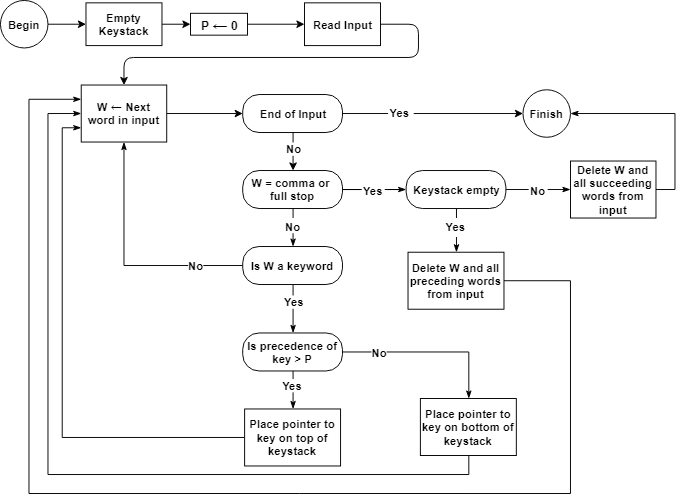
\includegraphics[width=\textwidth]{keyword-detection-flow}
	
	\caption{Flow diagram of keyword detection in ELIZA \autocite{weizenbaum-eliza1966}}
	\label{fig:keyword-detection-flow-diagram}
\end{figure} 
\noindent
Figure \ref{fig:keyword-detection-flow-diagram} above shows a simplified flow diagram of the process of keyword detection. The keystack is a stack data structure that holds all of the keys that are identified in the input. P is a pointer to a variable that holds the value of the highest key precedence that has been identified, whilst, W is a pointer to a variable that holds the current word in memory. In Weizenbaum's ELIZA, a comma or full stop was recognised as a delimiter and if the key stack was not empty, the rest of the input was discarded and the process of keyword identification ended. This process only cares about the key with the highest precedence, so if a key is found with a precedence value lower than P, then that key is placed on the bottom of the keystack.

\section{Psychology of conversation with chatterbots}
% talk about what type of conversation people talk about with chatterbots
%talk about architechture of chatbots (deloitte infographic) plus uses paper
The popularity and usability of chatterbots have increased with the technological advancements in \gls{nlp}, processing power available, machine learning models and the amount of data that is available to learn from \autocite{deloitte-chatbots2018}. To understand the psychology of conversation with chatterbots, the reasons why people use them and the types of conversations people have with them must be considered, as does the characteristics of the human brain a chatterbot must mimic to be considered successful.
\subsection{Uses of chatterbots}
The increase in engagement could be partly down to large companies, such as Microsoft, Facebook and Google, investing heavily into providing resources to developers to help them create chatterbots, quickly and more easily, and integrate them into social media platforms. For example, within a year of Facebook opening up their messaging platform, Facebook Messenger, to allow for chatterbot integration, more than 30,000 chatterbots had been developed and deployed \autocite{why-people-use-chatbots2017}. In a recent study researching why people use chatterbots, the majority of participants commented that they use chatterbots to increase their productivity. The other main categories the responses fell under were: entertainment, social/relational and novelty/curiosity \autocite{why-people-use-chatbots2017}. The responses that fell under the category of productivity felt that chatterbots allowed them to retrieve and access information more quickly and easily, which is one of the main applications of \gls{nlp}, known as information retrieval, discussed in sub-section \ref{ssection: nlp-applications}. Perhaps, most surprisingly, was the amount of people who responded that they often used chatterbots for entertainment and social/relational use. As the quality of chatterbots increase and become more human-like (which is the goal), people are interacting with chatterbots to alleviate boredom or as a outlet to relax, ``avoid loneliness" and ``improve social and conversational skills". Commercially, chatterbots are becoming popular as businesses look to make their customer services more efficient, innovative and, most importantly, more personal, due to the rising demand of customers looking for fast resolutions to their problems and the increase in time they are spending online \autocite{deloitte-chatbots2018}.
\subsection{Types of conversation with chatterbots}
A recent study found that the way people converse with chatterbots differs to the way people converse with another person \autocite{hill2015real}. It measured the differences in conversation between those with chatterbots and those with other humans among a number of categories, including use of profanity, length of messages and the use of shorthand and emojis. The study found that in general people conversed with chatterbots for a longer period of time, but on average the length of the messages was shorter. It also found that people used a much larger vocabulary with other humans as there was less diversity, in terms of the number of unique words used in a conversation with a chatterbot. The amount of profanity used in a conversation with a chatterbot was far greater than that with humans, which suggests that people feel safe to voice their true feelings with a chatterbot than with a human, which correlates to the research done by Brandtzaeg \& Følstad in their study on why people use chatterbots, which found that many people used chatterbots as a safe place to chat about their feelings \autocite{why-people-use-chatbots2017}.
\subsection{Characteristics of a chatterbot}
Different parts of the brain carry out different functions and so chatterbots can have different functionality mimicking different parts of the brain. Figure \ref{fig:deloitte-infographic} shows the different functions that the brain performs and how they relate to the architecture of a chatterbot. The three parts of the figure that this dissertation focusses on is: dialogue management (see section \ref{section: long-term-memory}), natural language processing (see section \ref{section: nlp}) and entity recognition (see section \ref{section: ner}). To be considered human-like, a chatterbot must try and mimic all parts of the brain as humans use all parts of the brain when conversing with other humans. From a commercial point of view, there are a number of characteristics that are important to consider when developing chatterbots \autocite{deloitte-chatbots2018}. Firstly, humans tend to engage more with chatterbots if they show human-like characteristics. One way this could be done is by developing the chatterbot to show emotion to the person it is conversing with. Weizenbaum's ELIZA tried to mimic emotion and the illusion of understanding by constructing responses in a way that it makes the person think that the chatterbot is understanding what they are saying. Another important characteristic is being able to reliably recognise the intent of the person chatting with the chatterbot. The chatterbot needs to be able to recognise what the user is asking for even if the message is phrased unusually, for example with spelling or grammatical errors. This is especially important in customer service chatterbots as you do not want to annoy the user.

\begin{figure}[h]
	\centering
	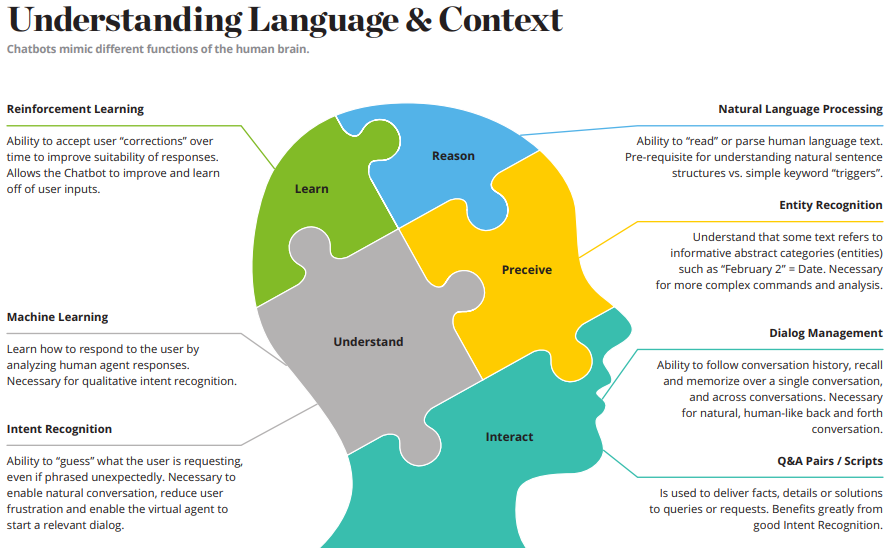
\includegraphics[width=\textwidth]{deloitte-infographic}
	\caption{Infographic showing the different functions of a chatterbot architecture \autocite{deloitte-chatbots2018}}
	\label{fig:deloitte-infographic}
\end{figure}
\section{Long-term memory and dialogue management} \label{section: long-term-memory}
% define LTM. Give examples of chatterbots with nlp. Introduce LSTMs.
As you can see in Figure \ref{fig:deloitte-infographic}, one of the techniques that a chatterbot can utilise to mimic the brain function to interact with other people is ``dialogue management". Dialogue management is concerned with building a mechanism to give the chatterbot the ability to control the flow of the conversation by interrupting the conversation flow at appropriate times to bring in knowledge that is outside of the current conversation. One way of managing the dialogue is by having a memory mechanism that stores the important parts of the conversation in a data structure and then refer back to this data structure at appropriate times to see if there is any knowledge that can be appropriately referred to in the current conversation flow. There are two types of memory mechanisms that can be used: long-term memory and short-term memory. Long-term memory is a way of recalling information into the current conversation from previous conversations. For example, if you were talking about going on a holiday with a friend, if you remember a memory of going on a holiday in the past, you can recall that information and talk about it in the current conversation. Short-term memory, on the other hand, is the ability to recall information that you have talked about in the current conversation.\\\\
In 1972, Tulving released an influential psychological insight into the different types of long-term memory \autocite{tulving1972episodic}. Three distinctive parts of long-term memory were identified: procedural, semantic and episodic memory \autocite{mcleod_2010}. Procedural memory is the part of the long-term memory responsible for remembering how to perform certain tasks (i.e. procedures). Semantic memory is a declarative form of memory responsible for remembering worldly and general knowledge, such as meanings of words or facts such as names of places. Finally episodic memory is responsible for remembering events that have occurred in our lives in the past.\\\\
A technique that has been used with various degrees of success is Hidden Markov chain models, which is a statistical model based on the probability of a word occurring in the input. For example, given the input, ``agggcagcgggcg", the markov model of order 1 predicts that the letter `g' will occur with a probability of 8/13 \autocite{bradevsko2012survey}. This technique is not suitable to be used with the ELIZA chatterbot due to the pattern matching and substitution technique the chatterbot employs. Markov models are much more suited to a chatterbot that has a more freely built conversation flow and chatterbots that perform certain actions when triggered by certain input.\\\\
Research that was found after the implementation of the product found another technique that is being used to solve the problem of long-term memory. This technique aims to solve the problem of mimicking the decentralised nature of the human brain, which with computers storing data in a centralised and structured manner was not possible. This technique uses a deep learning algorithm known as Recurrent Neural Networks, which can help memorise and retrieve data that has been processed. To process the data a algorithm called Neural Stack Machines is used to store the textual data in a suitable data structure.
\section{Natural Language Processing} \label{section: nlp}
% define what NLP is what it is used for
\gls{nlp} is a branch of \gls{ai} concerned with the research of natural language interactions between humans and computers. It has been defined in a number of ways, but the common aspects of all definitions is that \gls{nlp} involves the analysis and representation of naturally occurring language, at a number of levels of linguistic analysis, for the sole purpose of achieving the accuracy of language processing, on-par with humans, for a range of tasks \autocite{liddy2001natural}. Natural language has been defined in the white paper on \gls{nlp} as being ``the most natural means of communication between humans, and the mode of expression of choice for most of the documents they produce" \autocite{nlp-whitepaper1989} and this could be represented by written texts or spoken language.
\subsection{Levels of linguistic analysis}
Below are the 7 levels of linguistic analysis, from lowest to highest level of analysis, that a \gls{nlp} system can utilise \autocite{liddy2001natural}:
\begin{itemize}
	\item Phonology
	\item Morphology
	\item Lexical
	\item Syntactic
	\item Semantic
	\item Discourse
	\item Pragmatic
\end{itemize}
\textbf{Phonology} deals with interpreting different spoken sounds within and across words. This type of analysis takes into account sounds when words are spoken together as a sentence, individual word sounds, as well as, sounds when words are spoken with emphasis or when a person is stressed. When speech input is passed into an \gls{nlp} system, the sound waves are analysed and encoded into a digital signal, which is then interpreted by the rules employed by the system.\\
\textbf{Morphology} deals with breaking down words into its individual components. For example, the word ``preregistration" can be broken down into the following components: ``pre"(prefix), ``registra"(root) and ``tion"(suffix). This level of analysis is especially useful as the \gls{nlp} system can understand the context of conversation. For example, the word ``played" can be broken down into ``play" and ``ed". This provides information that this event happened in the past because of the suffix, ``ed".\\
\textbf{Lexical} analysis is concerned with understanding the meaning of individual words, but is not concerned with whether the words make sense in the context of the whole sentence. At this level of analysis, if a word can only have a single possible meaning in the context of the sentence, a semantic representation of this word can be made. Combining semantic representations across multiple words, can help provide complex insight into the meaning of sentences, as a whole, just as humans can produce this in their brains. See Figure \ref{fig:semantic-rep-nlp} for an example of a possible semantic representation of the word, ``launch".
\begin{figure}[H]
	\centering
	\hspace*{-2cm} 
	\begin{BVerbatim}
	launch (a large boat used for carrying people on rivers, lakes harbors, etc.)
	((CLASS BOAT) (PROPERTIES (LARGE)
	(PURPOSE (PREDICATION (CLASS CARRY) (OBJECT PEOPLE)))) 
	\end{BVerbatim}
	
	\caption{Example semantic representation of the word, ``launch" \autocite{liddy2001natural}}
	\label{fig:semantic-rep-nlp}
\end{figure}
\noindent
\textbf{Syntactic} analysis is concerned with analysing whole sentences to identify the grammatical structure that makes up that sentence and identify the dependencies between the words. This is important in most languages as the order words in a sentence can change dependencies and therefore the meaning of the sentence.\\ 
\textbf{Semantic} analysis is concerned with making decisions about the meanings of whole sentences by considering how the different semantic representations of the words, as dealt with in the lexical level, fit together. This level also deals with reducing ambiguity of words with multiple meanings. It does this by considering the context, in which the word appears in the sentence and/or considering domain knowledge if the scope of the \gls{nlp} system is limited.\\
\textbf{Discourse} analysis is concerned with analysing whole texts of documents to understand the meaning of the text as a whole. It does this by interpreting the interactions between the different sentences that makes up the text. The two most common discourse processing techniques that happen at this level are: anaphora resolution and discourse/text structure recognition. \textbf{Anaphora resolution} is concerned with replacing entities, such as pronouns, with the appropriate corresponding entity to which it refers. \textbf{Discourse/text structure recognition} is concerned with interpreting the purpose of a sentence in a document. This can help identify parts of a document that are meaningful or important or separate the document into different meaningful sections.\\
\textbf{Pragmatic} analysis is concerned with identifying the intentions of the author of the text and the wider context of the sentence in the document. This analysis requires a lot of understanding of world knowledge and intentions of speech in day-to-day conversations. For example, if someone asks another person to ``Draw the curtains", if the curtains are open you expect that person who is present to close the curtains, likewise, if the curtains are closed you expect that person to open the curtains \autocite[example taken from p. 5]{cam-nlp-linguistics}.

\subsection{Applications of Natural Language Processing} \label{ssection: nlp-applications}
The most common applications that involve \gls{nlp} can be grouped into the following categories \autocite{liddy2001natural}:
\begin{itemize}
	\item Information Retrieval
	\item Information Extraction
	\item Question-Answering
	\item Summarisation
	\item Machine Translation
	\item Dialogue Systems 
\end{itemize}
\noindent
\textbf{Information retrieval} is the task of finding material of an unstructured nature that satisfies a need of finding information from within large collections \autocite[pp. 1-4]{info-retrieval2018}. An example of an application of information retrieval is when you search for something on a search engine, such as Google, the query will return a list of links to pages that match your search term(s) closest.\\
\textbf{Information extraction} is the task of recognising, tagging and extracting key pieces of information into a structured format from large, unstructured collections of text \autocite{liddy2001natural}. Examples of the key pieces of information that this task will try and extract are: names of people, names of companies, geographical locations and names of products. A prominent technique that falls under this category is named entity recognition, which is discussed in section \ref{section: ner}.\\
\textbf{Question-answering} goes one step further than information retrieval by trying to provide a direct answer to a query rather than provide a list of relevant documents. An example of this is if you ask a question to a smart speaker, such as Amazon's Alexa-enabled devices, if it can provide a direct answer to your question it will use a third-party website to provide an answer to your question.\\
\textbf{Summarisation} is the task of reducing a large document into a smaller document. An example of an application of summarisation is that news aggregator apps or websites could summarise news articles to display a short summary of the news article, before users can click on the summary to see the full article.\\
\textbf{Machine translation} is the oldest task of \gls{nlp} and the goal is automatic translation of a text in one natural language into another, for example, English to Arabic, preserving the context and meaning of the original text as close as possible \autocite{stanford-nlp-mt}.\\
\textbf{Dialogue systems} is an area of \gls{nlp} with a lot of active research and the goal is to achieve human-like dialogue or conversation, whether that be using typed conversation or oral communication. 
\section{Named Entity Recognition} \label{section: ner}
% define ner and what are entities. Give comparison of tools that can be used for ner. Introduce CNNs and RNNs
\gls{ner} is a sub-task of \gls{nlp} concerned with identifying information units, know as entities, such as names of people, places, products and companies, as well as, numerical units, such as dates, times and monetary expressions \autocite{nadeau2007survey}, within textual documents. Figure \ref{fig:ner-entities} shows a visualisation of entities being extracted from a body of text.\\
\begin{figure}[h]
	\centering
	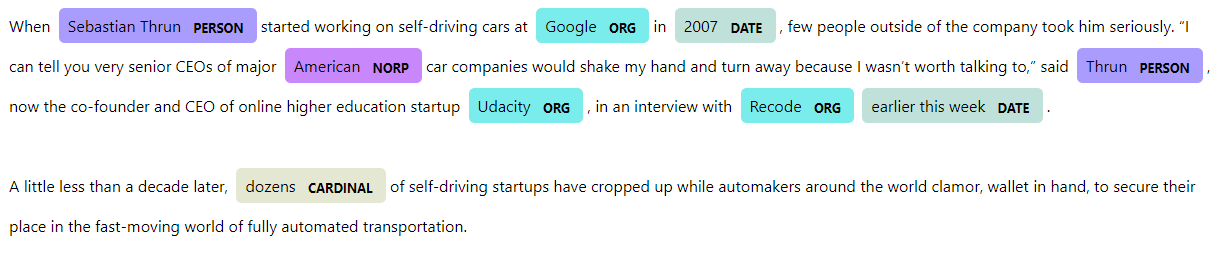
\includegraphics[width=\textwidth]{ner-entities}
	\caption{Figure showing a visual representation of entities being extracted from a body of text}
	\label{fig:ner-entities}
\end{figure}
\subsection{Named Entity Recognition Tools}
A study was completed comparing the leading tools and libraries for \gls{nlp} and \gls{ner} across a number of programming languages in 2015 \autocite{choi2015depends}. It found that overall spaCy had the best accuracy and speed when training and using their models. spaCy is also written in Cython, with a very high level wrapper written in Python making it easy to get started and apply an \gls{nlp} model. Python is also a simpler language to learn than a language like C++, where performance will be optimal, but it would take a long time to learn the language and implement the product. There are other libraries, like CoreNLP and StanfordNLP, but they are written in Java, which would require much more effort to write an application as it is a lower level wrapper. For prototyping, Python is one of the best languages as it has a simple syntax and a rich ecosystem of libraries, which are often high-level making it easy for beginners to get started.
\section{Summary}
This chapter introduced the reader to research that has been undertaken in the areas of chatterbots, psychology of conversation and \gls{nlp}. The next chapter will discuss the requirements of the product and the design decisions made prior to the start of the implementation phase.